\documentclass[11pt]{article}
\usepackage{amsmath}
\usepackage{amssymb}
\usepackage{fancyhdr}
\usepackage{tocloft}
\usepackage{graphicx}
\usepackage{calc}
\usepackage{amssymb}
\usepackage{color}
\usepackage[sc]{mathpazo}
\usepackage{url}
\usepackage{ifpdf}
\usepackage{bbding}
\usepackage{caption}
\usepackage{framed}
\usepackage{xcolor}
\usepackage{float}
\usepackage{wrapfig}
\usepackage{sidecap}
\linespread{1.0}
\oddsidemargin=0pt
\evensidemargin=0pt
\textwidth=6.5in
\topmargin=0pt
\headheight=0pt
\headsep=0pt
\textheight=9in
\setlength{\parindent}{0.25cm}
\newcommand\secfont{\fontfamily{cmss}\selectfont}%\textwidth 5.5truein
\newcommand\pifheading[1]{\noindent{\secfont\textbf{#1}:}}
\newcommand\yr{2016}
\def\lo{
\mathrel{\raise.3ex\hbox{$<$}\mkern-14mu\lower0.6ex\hbox{$\sim$}}
}
\def\hi{
\mathrel{\raise.3ex\hbox{$>$}\mkern-14mu\lower0.6ex\hbox{$\sim$}}
}

\textwidth = 6.5 in
\textheight = 9 in
\oddsidemargin = -0.00 in
\evensidemargin = +0.05 in
\topmargin = 0 in
\headheight = 0.0 in
\headsep = 0.0 in
\parskip = 0.05in

\newcommand\registered{{\ooalign{\hfil\raise .00ex\hbox{\scriptsize R}\hfil\crcr\mathhexbox20D}}}

%% Define a new 'leo' style for the package that will use a smaller font.
\makeatletter
\def\url@leostyle{%
  \@ifundefined{selectfont}{\def\UrlFont{\sf}}{\def\UrlFont{\small\ttfamily}}}
\makeatother
%% Now actually use the newly defined style.
\urlstyle{leostyle}
\newcommand\checkme[1]{\textcolor{blue}{\textbf{#1}}}
\newcounter{hours}\newcounter{minutes}
\newcommand\printtime{\setcounter{hours}{\time/60}\setcounter{minutes}{\time - \value{hours}*60}\thehours :\theminutes}
\newenvironment{packed_item}{
\begin{itemize}
 \setlength{\itemsep}{1pt}
 \setlength{\parskip}{0pt}
 \setlength{\parsep}{0pt}
}{\end{itemize}}

\newenvironment{packed_enum}{
\begin{enumerate}
 \setlength{\itemsep}{1pt}
 \setlength{\parskip}{0pt}
 \setlength{\parsep}{0pt}
}{\end{enumerate}}

\newenvironment{box_list}{
\begin{itemize}
 \setlength{\itemsep}{3pt}
 \setlength{\parskip}{0pt}
 \setlength{\parsep}{0pt}
}{\end{itemize}}

\newenvironment{packed_list}{
\begin{list}{\labelitemi}{\leftmargin=1em}
 \setlength{\itemsep}{3pt}
 \setlength{\parskip}{0pt}
 \setlength{\parsep}{0pt}
}{\end{list}}

\renewenvironment{quote}{%
  \list{}{%
    \leftmargin10pt   % this is the adjusting screw
    \rightmargin\leftmargin
  }
  \item\relax
}
{\endlist}

% definition of a new float type (refer to the caption package documentation)
\DeclareCaptionType{boxcaption}[Box]
\captionsetup[boxcaption]{position=top,labelfont=bf}

% definition of a shaded-like environment (see framed.sty)
\newenvironment{shadedframe}
  {\def\FrameCommand{\setlength\fboxsep{10pt}\fcolorbox{black}{shadecolor}}%
    \MakeFramed {\advance\hsize-\width \FrameRestore}}%
{\endMakeFramed}

\newenvironment{shadedbox}{%
  \def\FrameCommand{\colorbox{shadecolor}}%
  \MakeFramed {\FrameRestore}}%
 {\endMakeFramed}

% main environment
% syntax: \begin{myenv}{placement-specifiers}{color}{width}...\end{myenv}
\newenvironment{boxenv}[3]
  {\colorlet{shadecolor}{#2}%
    \begin{boxcaption}[#1]%
    \noindent\begin{minipage}{#3}
      \begin{shadedframe}
      }
  {\end{shadedframe}\end{minipage}\end{boxcaption}}

 % TOC
\usepackage{enumerate}
\begin{document}


\begin{figure}
  
\includegraphics[width=\linewidth/3]{title}
  \label{fig:title}
\end{figure}


\title{Lab Report 8: Operational Amplifiers II}


\author{Yuezhe Yao}

%\institute{Syracuse University}



\maketitle

\begin{abstract}
In this lab, and the corresponding reading assignment, we go beyond the 
Golden Rules and learn about some realistic characteristics of op amps, and, in the process, become familiar with more advanced op-amp operations.     
\end{abstract}

\medskip

\begingroup
\let\clearpage\relax
\tableofcontents
\endgroup

\medskip
\medskip

\section{Learning Objectives}

To become more familiar with op amp terminology, including parameters that characterize realistic op amp behavior like slew rate, settling time, open loop output impedance, and op amp instability.

To go beyond the Golden Rules and gain additional experience in op amp circuit design.

To learn how to use op amp circuits to shape and generate waveforms.

\section{Activity I - Op Amp Slew Rate and Settling Time}

Derive $\beta$:

For non-inverting amplifier, $V_{+}=V_{-}$

$V_{-}=\frac{R_{1}}{R_{1}+R_{2}}*V_{out}$

$\rightarrow the voltage gain \beta = {V_{out}\over V_{in}}={R_{1}\over R_{1}+R_{2}}$

The slew rate is inherently limited by the small internal drive currents of an op-amp but is also limited by internal capacitance designed to compensate against high frequency oscillations. Some op-amps are externally compensated and therefore offer some control over the slew rate. The formula to determine the minimum slew rate needed for a given frequency and output voltage is:

$S(in volts per second)=2\pi f*Required Peak Output Volts=2\pi fA_{p}$

$\rightarrow A_{p}\geq {S\over 2\pi f}$


\begin{figure}[H]
 \begin{center}
  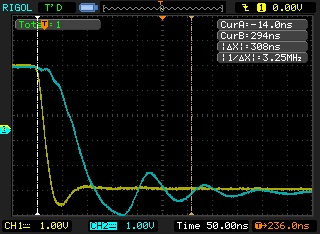
\includegraphics[width=\linewidth/1]{act1falling}
  \caption{The measurement of the falling time of the follower.}
  \label{fig:act1falling}
 \end{center}
\end{figure}

\begin{figure}[H]
 \begin{center}
  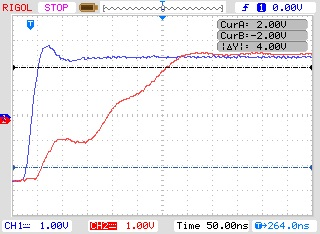
\includegraphics[width=\linewidth/1]{act1raising}
  \caption{The measurement of the rise time of the follower.}
  \label{fig:act1raising}
 \end{center}
\end{figure}

From our plots, we got the rise time is 254ns, and the Vpp is 5V, so the slew rate is $S=5V/254ns=19.7V/\mu s$, which is consistent with what we expect compared to the value $12V/\mu s$ come from the data sheet.

And the value of frequency for which distortion of the sinusoidal signal became noticeable is around 2.4MHz.

\begin{figure}[H]
 \begin{center}
  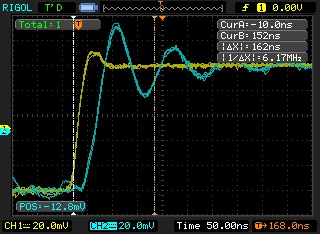
\includegraphics[width=\linewidth/2]{act1Gain1}
  \caption{The output signal response for the unity gain measurement of gain 1.}
  \label{fig:act1Gain1}
 \end{center}
\end{figure}

\begin{figure}[H]
 \begin{center}
  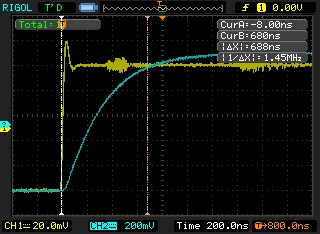
\includegraphics[width=\linewidth/2]{act1Gain11}
  \caption{The output signal response for the unity gain measurement of gain 11.}
  \label{fig:act1Gain11}
 \end{center}
\end{figure}

\begin{figure}[H]
 \begin{center}
  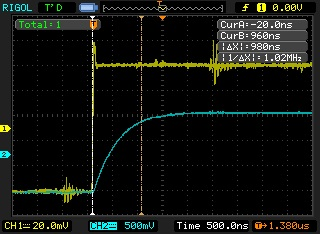
\includegraphics[width=\linewidth/1]{act1Gain16}
  \caption{The output signal response for the unity gain measurement of gain 16.}
  \label{fig:act1Gain16}
 \end{center}
\end{figure}

When gain=1, the settling time is 162ns, when gain=2,the settling time is 384ns, when gain=11, the settling time is 688ns, and when gain=16, the settling time is 980ns. The larger the gain, the more obvious the damping is. And by plug those values into equation (3), we found our results are consistent with the equation. For example, when gain=1, ft=2.4MHz, $t_{settle}=5*1/(2\pi *2.4)=331ns$


\section{Activity II - Frequency Compensation, Op Amp Output Impedance and Op-Amp Instability}


\begin{figure}[H]
 \begin{center}
  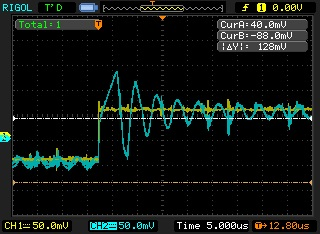
\includegraphics[width=\linewidth/1]{selfoscillation}
  \caption{self-oscillation.}
  \label{fig:selfoscillation}
 \end{center}
\end{figure}

We found that if we use the LF356, we couldn't observe the self oscillation. We saw the self oscillation when the instructor used another op-amp (AD829JN) after two weeks. We chose the capacitance as 1 $\mu$F, and we found that the implementation of a decoupling resistor (we chose 1 k$\Omega$) helps eliminate the oscillations. And for $\beta$:

$\beta = \frac{V_{-}}{V_{out}}=\frac{Z_{c}}{Z_{c}+R_{0}}=\frac{1}{1+i\omega R_{0}C}$

\section{Activity III - The Op Amp Comparator}

\begin{figure}[H]
 \begin{center}
  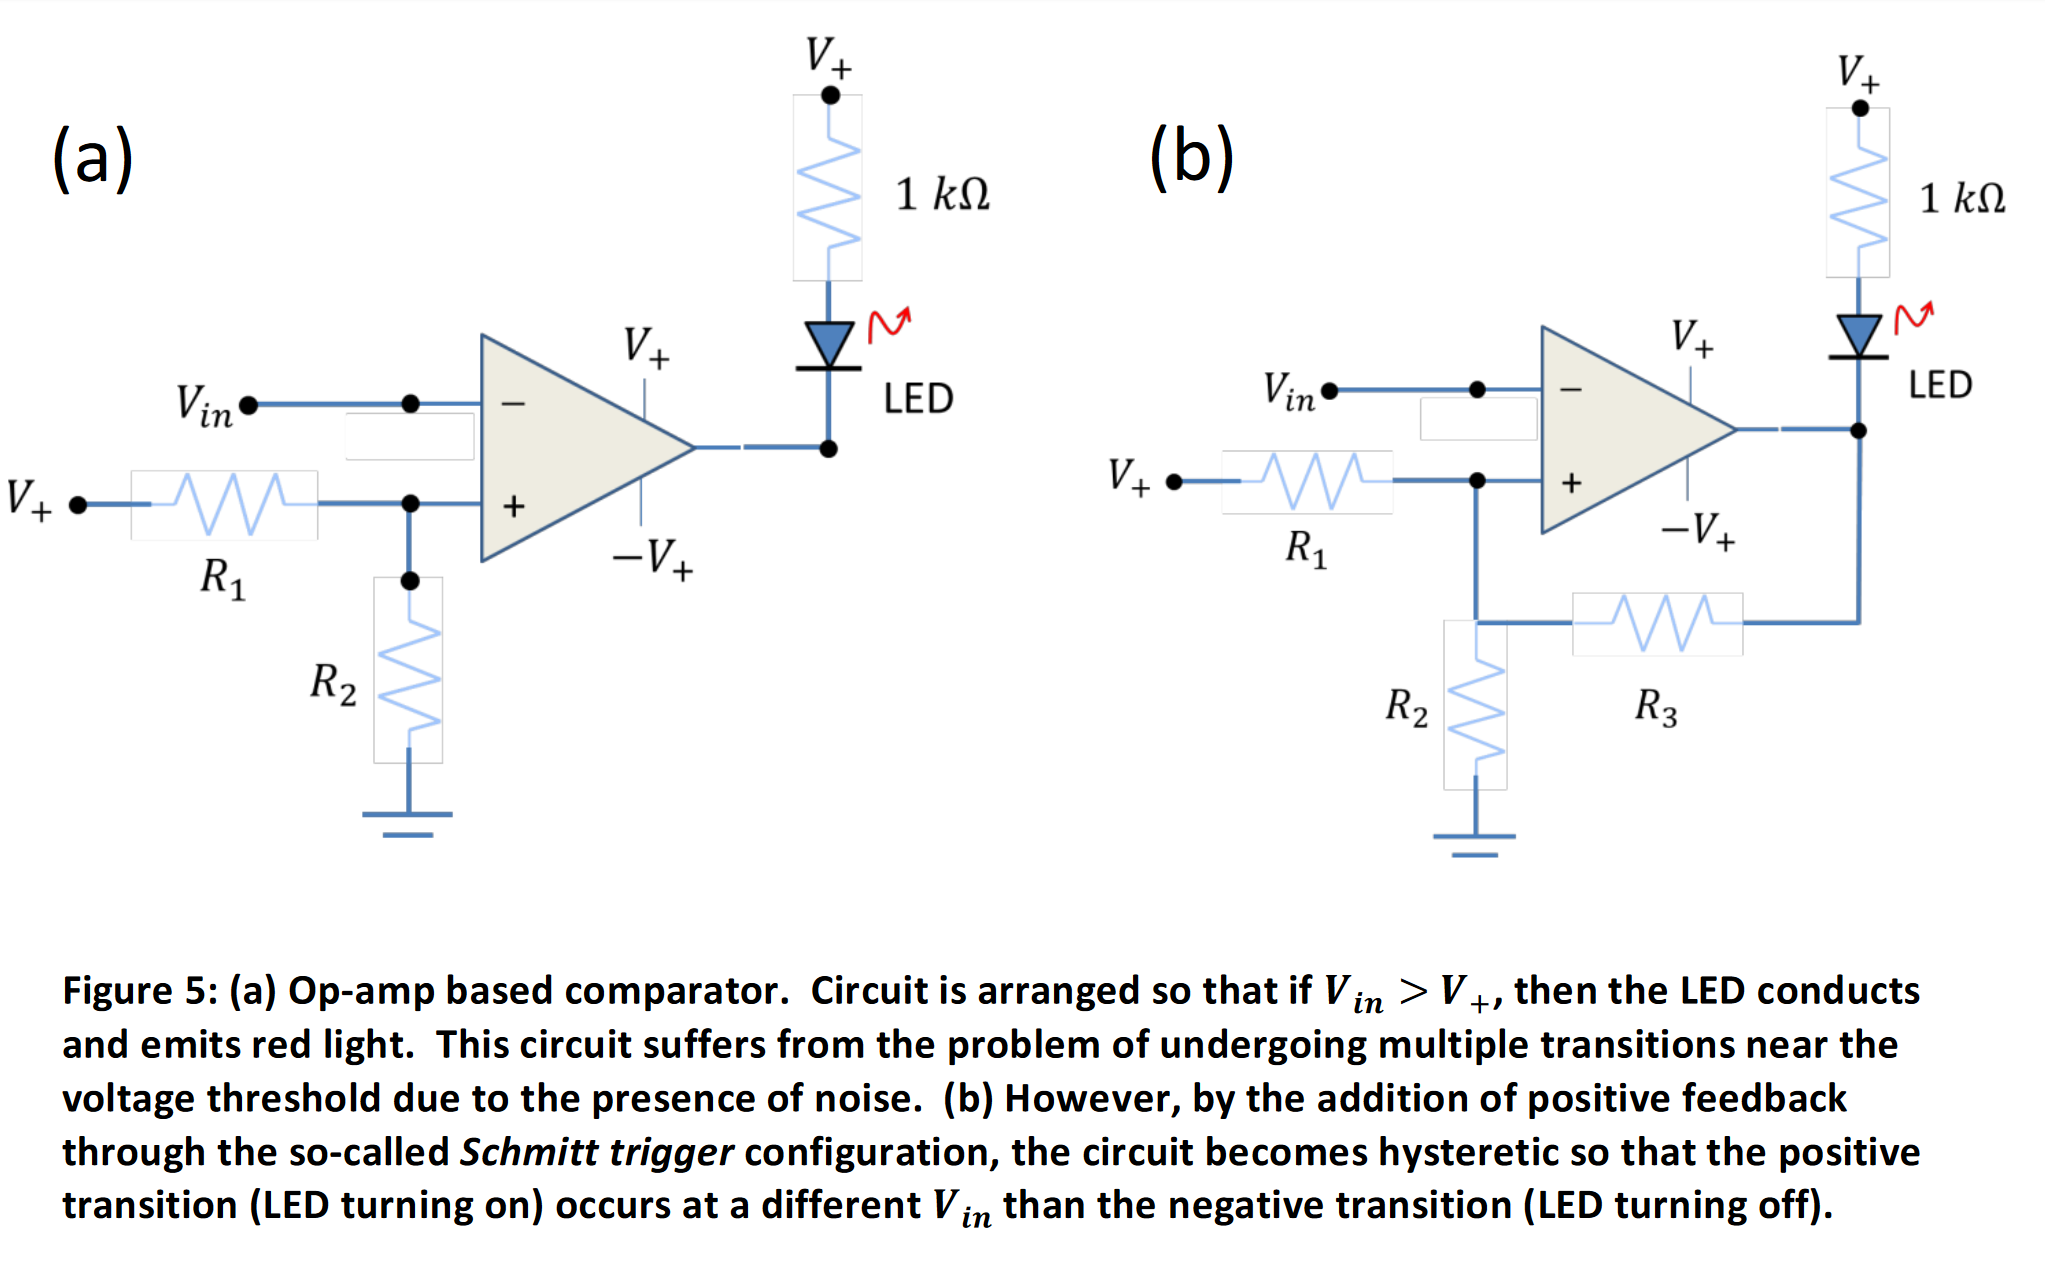
\includegraphics[width=\linewidth/1]{act3}
  \caption{}
  \label{fig:act3}
 \end{center}
\end{figure}

From the figure above, $V_{out}=A_{0}(V_{ref}-V_{in})$ ($V_{ref}$ is the voltage of the "+" terminal of the op-amp)

and $V_{ref}=V_{+}\frac{R_{2}}{R_{1}+R_{2}}$

$\Rightarrow if V_{+}\frac{R_{2}}{R_{1}+R_{2}}<V_{in}$, the LED will light up.

because the op-amp light up whenever $V_{in}>6V$, so

$V_{+}\frac{R_{2}}{R_{1}+R_{2}}<6V$

$\Rightarrow \frac{R_{2}}{R_{1}+R_{2}}<\frac{1}{2}$

$\Rightarrow$ we chose $R_{1}=R_{2}=1 k \Omega$

And we set $V_{pp}=2V, V_{DC}=4V$ as the offset, and the duration of the light became shorter.

\section{Activity IV - The Schmitt Trigger}

We found the equations in this website:

http://hyperphysics.phy-astr.gsu.edu/hbase/Electronic/schmitt.html\#c1

So now 

$V_{out1}=\frac{R_{123}}{R_{1}}V_{+}+\frac{R_{123}}{R_{3}}V_{cc}=6V$

$V_{out2}=\frac{R_{123}}{R_{1}}V_{+}-\frac{R_{123}}{R_{3}}V_{cc}=4V$

$V_{cc}=V_{+}=12V$

$R_{123}=R_{1}||R_{2}||R_{3}$

$\Rightarrow$ if we choose $R_{2}=1k\Omega$

$\Rightarrow R_{1}=1.2k\Omega, R_{3}=6k\Omega$

And our Schmitt Trigger worked well. We observed the hysteresis, in our lab, when $V_{in}>5.88V$, the light is on, when $V_{in}<4.2V$, the light is off. And when $4.2V < V_{in} < 5.88V$, whether the light is on or off depends on whether it was on or off. If it was on, then it'll keep on; if it was off, then it'll keep off.

\section{Activity V - Waveform Shaping with the Schmitt Trigger}

\begin{figure}[H]
 \begin{center}
  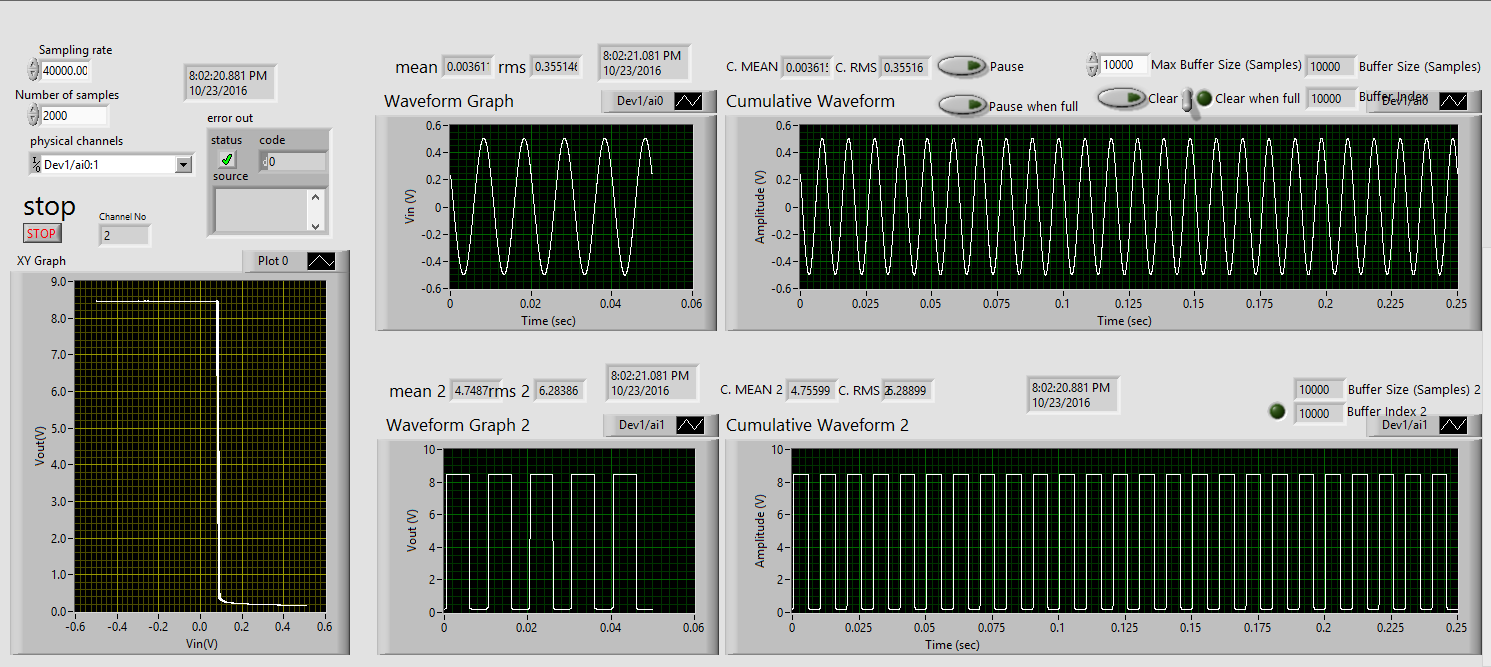
\includegraphics[width=\linewidth/1]{act5}
  \caption{Waveform shaping with the Schmitt Trigger}
  \label{fig:act5}
 \end{center}
\end{figure}


\vbox{}

From the figure above, we can see that the input signal is a sine wave and output is a square wave.

\begin{figure}[H]
 \begin{center}
  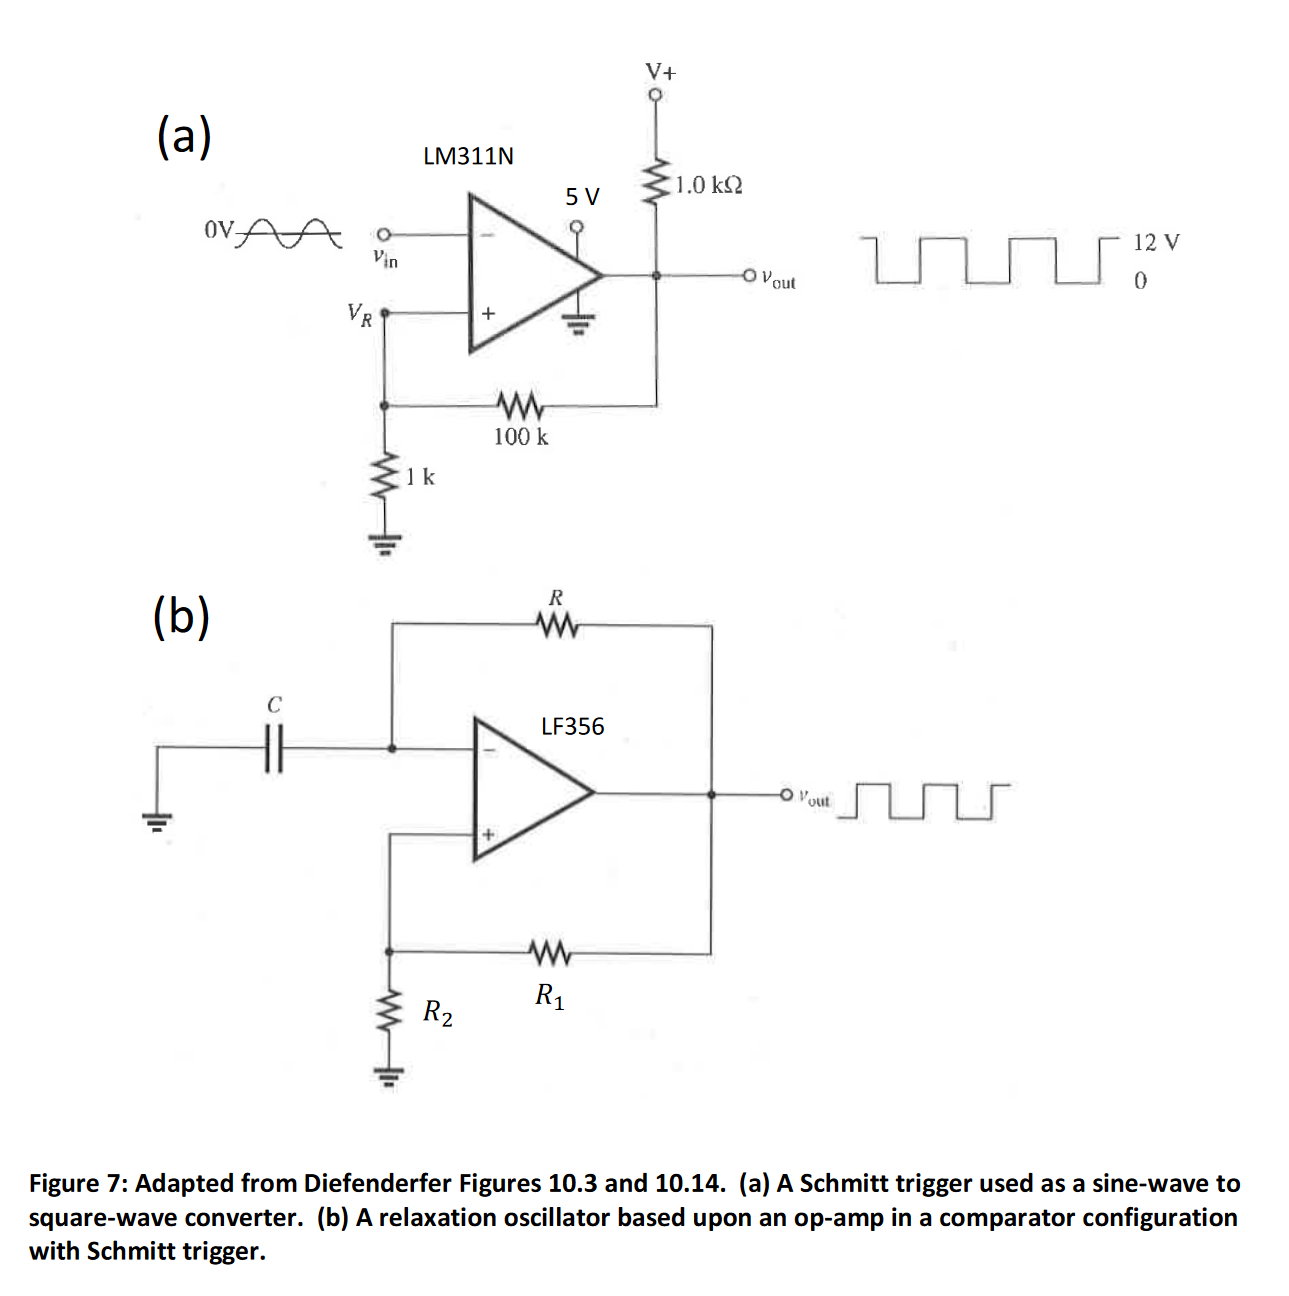
\includegraphics[width=\linewidth/1]{act56}
  \caption{}
  \label{fig:act56}
 \end{center}
\end{figure}

\vbox{}


Because of the positive feedback to the non-inverting input, the output is saturated in either the positive or negative direction. Assume the output is positively saturated, then a positive voltage is fed back to the non-inverting input voltage. This positive voltage is called upper trip point(UTP). As long as the inverting input voltage is less than UTP, the output voltage remains positively saturated. 

\vbox{}

If we slowly increase the input voltage, we eventually reach a point where it is slightly positive than the UTP. When this happens, the error voltage changes polarity, driving the op-amp into negative saturation. With the output now negative, the voltage divided feeds back a negative voltage to the non-inverting input. This negative voltage is referred to as the lower trip point(LTP).

\vbox{}

The output remains in negative saturation as long as the input voltage is more negative than the LTP. The only way to change the output is to decrease the input voltage until it is slightly more negative than LTP. Then the error voltage changes polarity and the output switches back to positive saturation.

\vbox{}

So one way to generate square wave is to drive a Schmitt trigger with a sine wave whose positive peak is greater than the UTP and whose negative is peak is less than the LTP. The shape of the input signal is immaterial. Instead of a sine wave, any periodic signal with sufficient amplitude to drive the Schmitt trigger will result in an output square wave.

\vbox{}

That's how it works.

\vbox{}

The reference comes from:

http://www.daenotes.com/electronics/digital-electronics/schmitt-trigger

\section{Activity VI - The Relaxation Square-Wave Oscillator}

\begin{figure}[H]
 \begin{center}
  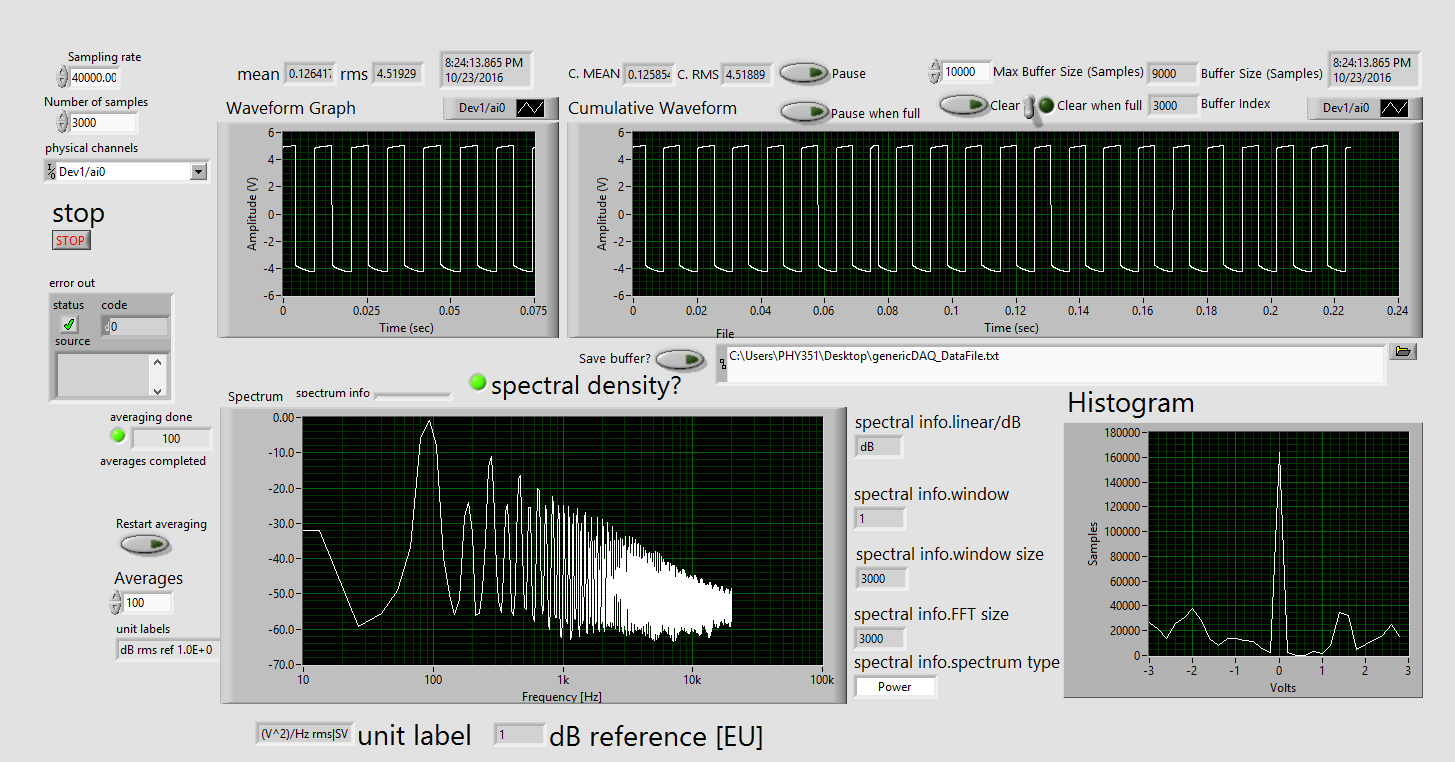
\includegraphics[width=\linewidth/1]{act6}
  \caption{The Relaxation Square-Wave Oscillator}
  \label{fig:act6}
 \end{center}
\end{figure}

From the picture above, we can see that the period is around 0.01s, and by using Eq.(4)

$T=2RCln[\frac{R_{1}+2R_{2}}{R_{1}}]=2*10^3\Omega*3.3*10^{-6}F*ln5=0.0106s$

which is consistent with our results.

The derivation of Eq.4:

let $\lambda=\frac{R_{2}}{R_{1}+R_{2}}$

When $V_{1}$ reaches $+\lambda V_{cc}$, then the switch to $-V_{cc}$ at the output occurs. The capacitor has charged to $+\lambda CV_{cc}$ and now begins to discharge. The general charging equation for a capacitor which already has an original charge is:

$q=CV[1-e^{-t/RC}]+q_{0}e^{-t/RC}$

For this case $V=-V_{cc}$ and $q_{0}=\lambda CV_{cc}$ so the charging equation is 

$q=CV_{cc}[1-e^{-t/RC}]+\lambda CV_{cc}e^{-t/RC}$

Now when q gets to $-\lambda V_{cc}$ another switch will occur. This time is half the period of the wave so it will be represented by T/2. At this time

$-\lambda CV_{cc}=-CV_{cc}[1-e^{-T/2RC}]+\lambda CV_{cc}e^{-T/2RC}$

$\Rightarrow T=2RCln[\frac{1+\lambda}{1-\lambda}]=2RCln[\frac{R_{1}+2R_{2}}{R_{1}}]$

We think the self-oscillating is because that the input voltage is easily affected by the adjacent rows.

\end{document}
